% Appendix for main.tex. Tables in tables/ are generated by scripts/make_tables.py from papers/analysis/*.json.

%==========================================================================================
\FloatBarrier
\section{Setup details}
\label{app:setup}

\paragraph{Pools.}
\Cref{tab:pools} lists every pool. Validity is decided by a program in all own-built pools and in MBPP and MATH-500; \textsc{MACE} entity questions use the benchmark's answer lists after a completeness audit (\cref{app:mace}), and the exploratory Ties pool uses an enumerated answer list known to be incomplete (\cref{app:ties}).
In own-built tasks, the reference is one member of the stored valid set, chosen by a seeded random draw when the task is built.

\begin{table}[h]
\centering
\small
\setlength{\tabcolsep}{4pt}
\begin{tabular}{L{2.6cm}L{5.2cm}L{2.5cm}L{2.4cm}}
\toprule
Pool & Contents & Generator & Judges \\
\midrule
Replication\osf & 120 tasks from five constraint families with exact checkers & Llama-3.1-8B-Instruct & Qwen2.5-7B, phi-4, Sonnet~5, GPT-4.1 \\
$k$-pool\osf & 75 tasks with exactly $k \in \{1,2,4,8,16\}$ valid answers, 15 per $k$; all 465 stored answers checked & Llama-3.1-8B-Instruct & Qwen2.5-7B, phi-4, Qwen2.5-14B, gemma-2-9b, Mistral-7B \\
Synthetic grid\pre & 60 tasks from two families whose valid sets enumerate exactly, 12 per $k$ & Qwen2.5-7B; Llama-3.1-8B & six open judges \\
Exploratory Ties & 51 generation tasks built from \textsc{RewardBench-2} Ties items & Qwen2.5-7B & Qwen2.5 1.5B--14B \\
\textsc{MACE}\pre & 300 questions with 1, 2, 4, or 6 correct answers (River, Language, and Math domains) & Llama-3.1-8B-Instruct & Qwen2.5-7B, phi-4, Sonnet~5 \\
MBPP\pre & 317 problems whose canonical solution passes the EvalPlus tests~\citep{liu2023evalplus} & Qwen2.5-7B & Qwen2.5-7B, 14B \\
MATH-500 & 105 problems with pass rate in $[0.2, 0.8]$, unique answers; the reference is the full MATH solution, or the final answer alone in \cref{app:estimator} & Qwen2.5-7B & Qwen2.5 1.5B--14B \\
Answer formats\pre & 25 new constraint tasks, each requested in four formats & Llama-3.1-8B-Instruct & Qwen2.5-7B, phi-4 \\
\bottomrule
\end{tabular}
\caption{Pools. Generators write 64 samples per task at temperature 1.0. The 37-task subset of \cref{app:frontier} is the $k$-pool tasks with both matching and non-matching valid samples; the 21-task subset of \cref{fig:mechanism} is the $k$-pool tasks with a single-number answer.}
\label{tab:pools}
\end{table}

\paragraph{Scoring.}
Open judges run in vLLM at temperature 0 and produce at most four tokens. We read the top-20 log-probabilities of the first generated token and take the probability-weighted mean over the score tokens 0 to 10, renormalized over their captured probability. For tokenizers that write ``10'' as the two tokens ``1'' and ``0'' (Qwen2.5, gemma-2, Mistral), the original scorer assigned all probability on ``1'' to the value 10 when the greedy reply began with ``10'' and to the value 1 otherwise. When less than 0.25 of the probability fell on score tokens, it used the integer in the greedy reply, or 5.0 if there was none. Mistral-7B's tokenizer has no single-token digits, so all of its scores, under either estimator, are the integers parsed from its greedy replies; phi-4 writes ``10'' as one token and is unaffected by the ``1'' rule. The pre-specified rescoring of \cref{app:estimator} replaces this rule with an exact two-step estimate: for each ``1'' token it runs one more forward step and splits that token's probability between 10 and 1 according to the probability of ``0'' next, and a reply with no score is treated as missing.
Sonnet~5 through the Anthropic API ran with extended thinking disabled and returns its score through a forced, schema-validated tool call. The command-line replication of \cref{sec:follows} replaced the tool's default system prompt with our rubric, disabled tools, and ran from an empty working directory (\cref{app:reasoning}); an earlier command-line run from the project directory is described in \cref{app:frontier}. GPT-4.1 uses the same expected-score estimator as the open judges, but its API returns at most five alternatives per token.

\paragraph{Selection accuracy and false rejection.}
For each task we select the sample with the highest rubric-$a$ score; when several samples tie at the maximum, accuracy is the mean validity of the tied samples. False rejection uses rubric-$a$ scores of oracle-valid samples whose extracted answer (the last \texttt{\textbackslash boxed\{\}} content, loosely normalized, or the whole reply if there is none) differs from the reference. Both are averaged per task and bootstrapped over tasks (1,000 resamples).

\paragraph{Inflation.}
For a task with samples $s_1,\dots,s_n$, let $a_i$ and $b_i$ be the rubric-$a$ and rubric-$b$ scores and $v_i \in \{0,1\}$ the validity. Select $s^\star = \arg\max_i a_i$, breaking ties at random, and compute
\begin{equation}
G \;=\; \frac{b_{s^\star}-\bar b}{\mathrm{sd}(b)} \;-\; \bigl(v_{s^\star}-\bar v\bigr).
\label{eq:gap}
\end{equation}
The null permutes the $a$-scores, and independently the $b$-scores, within the valid samples and within the invalid samples, recomputes $G$, and averages over 50 permutations. Inflation is $G$ minus this average. Permuting within validity classes leaves the largest $a$-score of each class unchanged, so the selected sample's validity class is the same under the null and the validity terms cancel. Inflation therefore equals the standardized rubric-$b$ score of the chosen sample minus the mean standardized rubric-$b$ score of samples with the same validity: how far above an average answer of the same correctness the chosen answer is scored. It is computed on tasks with pass rate in $[0.2, 0.8]$, where selection can change correctness, and reported as the referenced-minus-blind difference per task. Some analyses average over resampled sub-pools, as stated where they are used.

\paragraph{Prompts.}
The judge receives a system message with the rubric and a user message containing ``Problem:'', optionally ``Reference answer (trusted):'', and ``Candidate solution:'' followed by ``Score:''. The blind rubrics are:
\begin{quote}\small
(a) You are a strict grader. Read the question and the candidate response. Rate how correct and appropriate the response is on a scale from 0 (completely wrong or off-task) to 10 (fully correct). Judge the content, not the writing. Respond with only the integer score.\\[2pt]
(b) Evaluate the following response for correctness. Consider whether it actually answers the question asked. Ignore presentation quality. Give a single number from 0 to 10, where 0 means entirely incorrect and 10 means fully correct. Output only that number.
\end{quote}
The referenced rubrics are:
\begin{quote}\small
(a) You are a strict grader. You are given a question, a reference answer known to be correct, and a candidate response. Rate the candidate's correctness on a scale from 0 (completely wrong) to 10 (fully correct), using the reference to check it. Judge the content, not the writing. Respond with only the integer score.\\[2pt]
(b) Compare the candidate response against the trusted reference answer provided. Score how correct the candidate is, from 0 (entirely incorrect) to 10 (fully correct). Presentation does not matter. Output only a single number.
\end{quote}
The two instruction mitigations append one of these sentences to the referenced rubric:
\begin{quote}\small
Note: the reference shown is one valid answer among possibly many; the question may have several correct answers, and any correct answer deserves full credit even if it differs from the reference.\\[2pt]
Important: do not compare the candidate's answer to the reference. Use the reference only to understand the problem. Verify the candidate's answer on its own merits; a correct answer that differs from the reference must receive the same score as one that matches it.
\end{quote}
Blind-then-reveal first scores the candidate with the blind rubric. The second call appends to the referenced rubric: ``You have already assessed this candidate without seeing any reference. A correct answer that differs from the reference must keep the score you gave it; revise only if the reference reveals the candidate is actually wrong.'' Its user message shows the reference as ``Reference answer (one valid answer, trusted)'' and ends with ``Your blind score for this candidate was $x$ out of 10.'' In the neutral-wording variant this line reads ``A previous blind assessment scored this candidate $x$ out of 10.'' On MATH-500 the second call shows the trusted reference solution and says that a correct solution that differs from the reference ``in method or presentation'' keeps its score.

%==========================================================================================
\FloatBarrier
\section{Preregistration ledger}
\label{app:ledger}

Every confirmatory prediction was written down before its data existed. Three experiments were registered on OSF with third-party timestamps\osf{} (links withheld for review; anonymized copies are in the supplementary material). The rest were committed to the project repository with a timestamp that predates the data\pre. Analyses marked post hoc\ph{} carry no registration weight. \Cref{tab:ledger} lists every experiment and its outcome as scored. Counting each prediction once, the ledger records 46 confirmed, 24 falsified or failed, and 10 split, partial, inconclusive, not evaluable, or not scored.

{\small
\setlength{\tabcolsep}{4pt}
\begin{longtable}{L{3.3cm}L{0.9cm}L{8.9cm}}
\caption{Every registered experiment and its outcome.}\label{tab:ledger}\\
\toprule
Experiment & Record & Predictions and outcome \\
\midrule
\endfirsthead
\multicolumn{3}{l}{\small\emph{\cref{tab:ledger}, continued}} \\
\toprule
Experiment & Record & Predictions and outcome \\
\midrule
\endhead
\bottomrule
\endfoot
Replication (\cref{sec:selection}) & OSF & Reference adds inflation (\textbf{confirmed}); picks collapse onto the key (\textbf{confirmed}); positive margin (\textbf{confirmed}). Post hoc: accuracy, false rejection, selection pressure, population sensitivity. \\
$k$-pool and mitigations (\cref{sec:selection,sec:fix}) & OSF & Step from $k{=}1$ to $k{>}1$ positive (\textbf{confirmed}); blind-then-reveal lowers inflation at $k{>}1$ (\textbf{confirmed}); blind-then-reveal preserves the $k{=}1$ benefit (\textbf{partial}: no measurable cost; the benefit itself did not appear). The validity gate was registered as a hard gate and run as a soft multiplier, disclosed in a public amendment. Post hoc: accuracy readouts. \\
Judge coverage (\cref{app:mitigation}) & OSF & Every added judge shows harm (\textbf{not confirmed}: Mistral-7B null, a score-resolution artifact); blind-then-reveal lowers inflation for every added judge (\textbf{confirmed} as first scored; for Mistral-7B the upper interval bound of this contrast crosses zero in 3 of 8 reruns of the analysis, which is not fully deterministic). \\
Exploratory Ties study (\cref{app:ties}) & git & The registered population left 7 tasks; full-pool and pooled estimators were chosen after seeing data (disclosed). \\
Rotation, Ties pool (\cref{app:rotation}) & git & Same-sample gain under rotation (\textbf{confirmed}, all four sizes). \\
Rotation, replication pool (\cref{sec:follows}) & git & Gain, loss, and gain above placebo (\textbf{confirmed}, 12 of 12 cells). \\
Blind-accepted filter (\cref{sec:follows}) & git & Effect survives on answers scored $\geq 7$ blind (\textbf{confirmed}). \\
Synthetic grid (\cref{app:grid}) & git & Inflation higher with the reference at $k{>}1$ (\textbf{confirmed} in direction, six judges); anchoring margins grow with $k$ (\textbf{falsified} for the weaker judges). Post hoc: paired step and slope estimates. \\
Instruction, second wording (\cref{sec:fix}) & git & Same ordering of judges as the first wording (\textbf{confirmed}). \\
Composition dose (\cref{app:composition}) & git & Inflation rises with the number of matching valid answers (\textbf{falsified}: it falls). \\
Constructed lure test & git & Closed without judging after its naturalness audit failed in five rounds. \\
Two-factor composition (\cref{app:composition}) & git & Lures raise inflation at $d{=}0$ (\textbf{split}); removing lures restores a rising dose response (\textbf{falsified}); lures lower the valid-pick rate (\textbf{confirmed}); the selection model reproduces the surface (\textbf{confirmed}). \\
Distance gradient (\cref{app:composition}) & git & Penalty grows with distance from the reference (\textbf{falsified}, both judges). \\
Masking suite (\cref{sec:mechanism}) & git & Words preserve the margin, expression shrinks it, masking removes it (\textbf{confirmed}, 6 of 6 cells). \\
Worked reference (\cref{app:mitigation}) & git & Differs from a bare reference, sign not predicted (\textbf{confirmed}: milder). \\
Solution-route rotation (\cref{app:mechanism}) & git & Interval containing zero (\textbf{falsified} as stated: three of four cells exclude zero, with effects 20 to 400 times smaller than answer rotation). \\
\textsc{MACE} (\cref{app:mace}) & git & Step positive on audited domains, help at $k{=}1$, same sign in the math control (\textbf{confirmed}, 3 of 3). \\
Frontier CLI judge (\cref{app:frontier}) & git & Judge anchors (\textbf{confirmed}); blind margin null (\textbf{confirmed}); margin smaller than the open judges' (\textbf{not interpretable}: different score interface). \\
Frontier API judges (\cref{app:frontier}) & git & Rotation, filter, masking, and \textsc{MACE} results reproduce on Sonnet~5 (\textbf{confirmed}); GPT-4.1 passes the score-resolution screen (\textbf{failed}); GPT-4.1 $k$ step on two pools (\textbf{not confirmed}, ties); instructions shrink the margin on both (\textbf{confirmed}). A parsing fault in the first Sonnet~5 collection was found; all Sonnet~5 data were discarded and recollected, and only recollected data are reported. \\
Code exemplar (\cref{app:code}) & git & Canonical solution inflates like a key (\textbf{falsified}); a small similarity bias remains (\textbf{confirmed}). \\
Answer-format continuum (\cref{app:code}) & git & Attenuation from integer to program (\textbf{confirmed}); null at the program format (\textbf{confirmed} phi-4, \textbf{falsified} Qwen2.5-7B); margins at pair and JSON (\textbf{not evaluable}). A checker bug found after registration was fixed; no verdict changed. \\
Reveal-call variants (\cref{sec:fix}) & git & Removing the score restores inflation (\textbf{confirmed}); neutral wording equivalent (\textbf{confirmed} phi-4, \textbf{falsified} Qwen2.5-7B); another judge's score equivalent (\textbf{confirmed}). \\
Variants on gemma-2-9b (\cref{app:mitigation}) & git & Removing the score restores inflation (\textbf{confirmed}); neutral wording inert (\textbf{confirmed}); another judge's score equivalent (\textbf{falsified}). \\
Training, runs 1--3 (\cref{app:dpo}) & git & Reference arm passes its check (\textbf{confirmed}, runs 1 and 3); reveal and blind arms pass theirs (\textbf{failed}); reference arm copies the key more (\textbf{falsified}). A pre-adopted stopping rule closed the mitigation and attribution questions as unresolved. \\
Decode cost (\cref{app:mechanism}) & git & Margin survives one step (\textbf{falsified}); graded decline (\textbf{split}); below half at three steps (\textbf{confirmed}); inflation non-increasing (\textbf{split}). \\
Compression weight on gemma (\cref{app:mitigation}) & git & Lower than both other judges (\textbf{confirmed}, 4 tasks). \\
Constraint-problem pilot and follow-ups (\cref{app:mathconstraint}) & git & Solve rate, rotation, margin (\textbf{confirmed}); rotation on all six answer pairs, lure effect, Sonnet~5 (\textbf{confirmed}); selection harm, four designs (\textbf{falsified}; \textbf{inconclusive}; \textbf{falsified}, with the reference's own text among the candidates; \textbf{not confirmed}, right direction for both judges on 8 items). \\
Blind-then-reveal on MATH-500 (\cref{sec:fix}) & git & Reference raises accuracy over blind (\textbf{confirmed}, without registration weight after a disclosed amendment); the protocol keeps less than half of that benefit (\textbf{falsified}: it keeps nearly all of it). \\
Judges that write first: MT-Bench template (\cref{sec:reasoning}) & git & Rotation gain (\textbf{confirmed}); rotation loss (\textbf{confirmed}); referenced margin above blind at $k{>}1$ (\textbf{confirmed}); accuracy step below zero (\textbf{confirmed}). \\
Judges that write first: thinking judge (Qwen3-8B) (\cref{app:rotation}) & git & Rotation gain (\textbf{falsified}); rotation loss (\textbf{falsified}); referenced margin above blind at $k{>}1$ (\textbf{falsified}); accuracy step below zero (\textbf{falsified}). No measurable anchoring. \\
Thinking on versus off, same weights (Qwen3-8B; \cref{sec:reasoning}) & git & Thinking off: rotation loss (\textbf{confirmed}); rotation gain (\textbf{confirmed}); referenced margin above blind at $k{>}1$ (\textbf{confirmed}). Loss smaller with thinking on (\textbf{confirmed}). \\
Thinking judge on factual questions (\textsc{MACE}; \cref{sec:reasoning}) & git & Referenced margin above blind with thinking on (\textbf{confirmed}) and off (\textbf{confirmed}); smaller with thinking on (\textbf{confirmed}). \\
Sonnet~5 with and without thinking, CLI (\cref{app:reasoning}) & git & Score-only arm anchors under rotation (\textbf{confirmed}). Thinking and visible-reasoning arms smaller loss, and thinking fewer false rejections (\textbf{not scored}: stopped by the subscription's usage limit before data were complete). \\
\textsc{MACE} end to end (\cref{sec:selection,app:reasoning}) & git & Reference lowers accuracy at $k{>}1$ (\textbf{falsified}, both judges); blind-then-reveal beats the reference at $k{>}1$ (\textbf{falsified}); blind-then-reveal at least as accurate pooled over the natural mix (\textbf{falsified}). \\
Step-level rotation pilot & git & Registered; not scored at the time of writing. \\
\end{longtable}
}

%==========================================================================================
\FloatBarrier
\section{Rotation: all cells and the judge-size ladder}
\label{app:rotation}

The rotation assigns each task the valid alternative that appears most often among its valid samples, so that enough samples match the new reference. This choice makes cross-sample margins partly reflect how common an answer is; the paired same-sample changes in \cref{tab:rotation} compare each sample with itself and are not affected.

\begin{table}[h]
\centering
\footnotesize
\setlength{\tabcolsep}{3pt}
\begin{adjustbox}{max width=\linewidth}\begin{tabular}{llcccc}
\toprule
Judge & Rubric & Moved onto ($n{=}120$) & Moved off ($n{=}93$) & Neither ($n{=}113$) & Onto minus neither \\
\midrule
Qwen2.5-7B & $a$ & $+4.97$ {\scriptsize$[+4.66,+5.27]$} & $-5.04$ {\scriptsize$[-5.38,-4.67]$} & $+0.13$ {\scriptsize$[-0.04,+0.31]$} & $+4.81$ {\scriptsize$[+4.44,+5.17]$} \\
 & $b$ & $+6.34$ {\scriptsize$[+6.10,+6.60]$} & $-6.58$ {\scriptsize$[-6.89,-6.26]$} & $+0.10$ {\scriptsize$[-0.11,+0.29]$} & $+6.18$ {\scriptsize$[+5.84,+6.50]$} \\
phi-4 & $a$ & $+4.09$ {\scriptsize$[+3.79,+4.38]$} & $-3.92$ {\scriptsize$[-4.26,-3.59]$} & $+0.30$ {\scriptsize$[+0.04,+0.57]$} & $+3.88$ {\scriptsize$[+3.52,+4.25]$} \\
 & $b$ & $+3.25$ {\scriptsize$[+2.95,+3.51]$} & $-3.18$ {\scriptsize$[-3.46,-2.87]$} & $+0.24$ {\scriptsize$[+0.01,+0.47]$} & $+3.08$ {\scriptsize$[+2.76,+3.41]$} \\
Claude Sonnet 5 & $a$ & $+3.04$ {\scriptsize$[+2.53,+3.56]$} & $-2.66$ {\scriptsize$[-3.36,-2.00]$} & $+0.04$ {\scriptsize$[-0.41,+0.46]$} & $+3.08$ {\scriptsize$[+2.45,+3.78]$} \\
 & $b$ & $+2.54$ {\scriptsize$[+2.04,+3.08]$} & $-2.51$ {\scriptsize$[-3.17,-1.89]$} & $+0.28$ {\scriptsize$[-0.10,+0.69]$} & $+2.31$ {\scriptsize$[+1.75,+2.86]$} \\
\quad blind-certified only & $a$ & $+2.79$ {\scriptsize$[+2.26,+3.40]$} & $-2.50$ {\scriptsize$[-3.20,-1.83]$} & $+0.20$ {\scriptsize$[-0.21,+0.65]$} & $+2.67$ {\scriptsize$[+2.04,+3.33]$} \\
\bottomrule
\end{tabular}
\end{adjustbox}
\caption{Change in score of identical text when the reference is rotated (replication pool, 0--10 scale, 95\% CI). ``Onto'': samples that match the new reference. ``Off'': samples that matched only the old one. ``Neither'': valid samples matching neither. The last row keeps only samples Sonnet~5 scored at least 7 blind (3,194 of 3,494). For the open judges the same filter gives $+4.99$ \ci{+4.69}{+5.32} (Qwen2.5-7B, 91\% kept) and $+4.08$ (phi-4, 98\% kept).\pre}
\label{tab:rotation}
\end{table}

Before the replication, we ran the same test on the exploratory Ties pool at four Qwen2.5 judge sizes (\cref{tab:ladder}). The effect is largest for small judges, where it saturates the scale, and smaller but present at 14B. On the same split, blind margins are small, and samples matching neither reference move between $-0.44$ and $+0.82$. Restricting to samples the 7B judge scored at least 7 blind gives $+4.74$ \ci{+3.67}{+5.87} against $+4.57$ unfiltered.

\begin{table}[h]
\centering
\footnotesize
\setlength{\tabcolsep}{4pt}
\begin{tabular}{llcccc}
\toprule
Readout & Rubric & 1.5B & 3B & 7B & 14B \\
\midrule
Gain, reference moved onto the sample ($n{=}40$) & $a$ & $+9.48$ & $+9.29$ & $+4.57$ & $+3.07$ \\
 & $b$ & $+8.73$ & $+9.58$ & $+5.96$ & $+3.47$ \\
Loss, reference moved off the sample ($n{=}10$) & $a$ & $-9.65$ & $-8.85$ & $-3.14$ & $-2.78$ \\
 & $b$ & $-9.42$ & $-9.80$ & $-4.71$ & $-3.81$ \\
Referenced margin ($n{=}18$) & $a$ & $+9.00$ & $+9.05$ & $+4.75$ & $+3.26$ \\
 & $b$ & $+8.36$ & $+9.12$ & $+5.93$ & $+3.67$ \\
Blind margin, same split ($n{=}18$) & $a$ & $+0.16$ & $+1.36$ & $+0.31$ & $+0.69$ \\
 & $b$ & $+0.61$ & $+1.91$ & $+0.14$ & $+0.04$ \\
\bottomrule
\end{tabular}
\caption{Rotation on the exploratory Ties pool, Qwen2.5 judges (0--10 scale).\pre}
\label{tab:ladder}
\end{table}

\paragraph{Judges that explain or think before scoring.}
A later pre-specified experiment re-ran the rotation on a subsample of the replication pool (up to three samples per class per task, 879 samples) and the $k$ comparison on a 16-sample subsample of the $k$-pool, under two protocols: the verbatim MT-Bench single-answer templates with Qwen2.5-7B (the reference version asks the judge to begin ``by comparing the assistant's answer with the reference answer'' and to explain before a rating from 1 to 10), and Qwen3-8B with thinking enabled (temperature 0.6, up to 4,096 new tokens, rubric~$a$ ending in a ``Score: N'' line). Replies without a parseable score were dropped (20 of 879 rotation pairs for MT-Bench; none for the thinking judge's rotation replies). \Cref{tab:r2b} gives the results; accuracy is best-of-16.

\begin{table}[h]
\centering
\footnotesize
\setlength{\tabcolsep}{3pt}
\begin{adjustbox}{max width=\linewidth}\begin{tabular}{lcccccc}
\toprule
Protocol & Moved onto & No longer matches & Neither & Margin, $k{>}1$ (ref $-$ blind) & Accuracy, $k{=}1$ & Accuracy, $k{>}1$ \\
\midrule
MT-Bench template, Qwen2.5-7B & $+3.618$ {\scriptsize$[+3.401,+3.842]$} & $-3.591$ {\scriptsize$[-3.936,-3.242]$} & $+0.077$ {\scriptsize$[-0.212,+0.404]$} & $+3.19$ {\scriptsize$[+2.57,+3.88]$} & $+16.6$ {\scriptsize$[-1.5,+34.2]$} & $-13.0$ {\scriptsize$[-25.1,-1.1]$} \\
Thinking judge, Qwen3-8B & $-0.006$ {\scriptsize$[-0.017,+0.000]$} & $+0.011$ {\scriptsize$[+0.000,+0.032]$} & $-0.003$ {\scriptsize$[-0.009,+0.000]$} & $+0.06$ {\scriptsize$[-0.10,+0.26]$} & $-5.8$ {\scriptsize$[-11.4,-1.8]$} & $-3.7$ {\scriptsize$[-7.5,+0.0]$} \\
\bottomrule
\end{tabular}
\end{adjustbox}
\caption{Judges that write before scoring: change in score of identical text under rotation (points, 95\% CI).\pre}
\label{tab:r2b}
\end{table}

\begin{table}[h]
\centering
\footnotesize
\begin{adjustbox}{max width=\linewidth}\begin{tabular}{lccc}
\toprule
Protocol & Margin, $k{>}1$ (ref $-$ blind) & Accuracy change, $k{=}1$ & Accuracy change, $k{>}1$ \\
\midrule
MT-Bench template, Qwen2.5-7B & $+3.19$ {\scriptsize$[+2.57,+3.88]$} & $+16.6$ {\scriptsize$[-1.5,+34.2]$} & $-13.0$ {\scriptsize$[-25.1,-1.1]$} \\
Thinking judge, Qwen3-8B & $+0.06$ {\scriptsize$[-0.10,+0.26]$} & $-5.8$ {\scriptsize$[-11.4,-1.8]$} & $-3.7$ {\scriptsize$[-7.5,+0.0]$} \\
\bottomrule
\end{tabular}
\end{adjustbox}
\caption{Judges that write before scoring on the 16-sample $k$-subsample: referenced-minus-blind anchoring margin at $k{>}1$ (points) and change in best-of-16 selection accuracy (points, 95\% CI).\pre}
\label{tab:r2b-k}
\end{table}
The thinking judge gives a score of 10 to 96.2\% of valid rotation samples blind and to 99.8\% with either reference, while invalid $k$-subsample answers average 3.67 blind and 3.15 with the reference; it writes 569 to 1,092 tokens on average, and 82.7\% of its referenced rotation replies mention the reference in their final text. Under the MT-Bench template, by contrast, the mean score of valid rotation samples falls from 6.68 blind to 4.97 with the reference. These diagnostics are post hoc.

%==========================================================================================
\FloatBarrier
\section{Selection: accuracy by pool and by $k$}
\label{app:grid}

\begin{table}[h]
\centering
\footnotesize
\setlength{\tabcolsep}{3pt}
\begin{adjustbox}{max width=\linewidth}\begin{tabular}{llcccccc}
\toprule
Judge & Protocol & $k{=}1$ & $k{=}2$ & $k{=}4$ & $k{=}8$ & $k{=}16$ & pooled $k{>}1$ \\
\midrule
Qwen2.5-7B & reference & $-21.4$ {\scriptsize$[-42.9,+0.0]$} & $-23.1$ {\scriptsize$[-53.8,+7.7]$} & $-11.1$ {\scriptsize$[-33.3,+0.0]$} & $-30.0$ {\scriptsize$[-60.0,+0.0]$} & $-71.4$ {\scriptsize$[-100.0,-42.9]$} & $-30.8$ {\scriptsize$[-46.2,-17.9]$} \\
 & blind, then reveal & $-21.4$ {\scriptsize$[-42.9,+0.0]$} & $-15.4$ {\scriptsize$[-46.2,+15.6]$} & $-11.1$ {\scriptsize$[-33.3,+0.0]$} & $-10.0$ {\scriptsize$[-30.0,+0.0]$} & $+0.0$ {\scriptsize$[-42.9,+42.9]$} & $-10.3$ {\scriptsize$[-25.6,+5.1]$} \\
 & validity gate & $+0.0$ {\scriptsize$[+0.0,+0.0]$} & $+15.4$ {\scriptsize$[+0.0,+38.5]$} & $+0.0$ {\scriptsize$[+0.0,+0.0]$} & $-10.0$ {\scriptsize$[-30.0,+0.0]$} & $-28.6$ {\scriptsize$[-57.1,+0.0]$} & $-2.6$ {\scriptsize$[-12.8,+7.7]$} \\
\addlinespace
phi-4 & reference & $+0.0$ {\scriptsize$[+0.0,+0.0]$} & $+0.0$ {\scriptsize$[+0.0,+0.0]$} & $+0.0$ {\scriptsize$[-33.3,+33.3]$} & $-20.0$ {\scriptsize$[-50.0,+0.0]$} & $-85.7$ {\scriptsize$[-100.0,-57.1]$} & $-20.5$ {\scriptsize$[-35.9,-5.1]$} \\
 & blind, then reveal & $-14.3$ {\scriptsize$[-35.7,+0.0]$} & $+0.0$ {\scriptsize$[+0.0,+0.0]$} & $+0.0$ {\scriptsize$[-33.3,+33.3]$} & $-20.0$ {\scriptsize$[-50.0,+0.0]$} & $-57.1$ {\scriptsize$[-85.7,-14.3]$} & $-15.4$ {\scriptsize$[-28.2,-2.6]$} \\
 & validity gate & $-7.1$ {\scriptsize$[-21.4,+0.0]$} & $+0.0$ {\scriptsize$[+0.0,+0.0]$} & $+0.0$ {\scriptsize$[+0.0,+0.0]$} & $+0.0$ {\scriptsize$[+0.0,+0.0]$} & $+0.0$ {\scriptsize$[+0.0,+0.0]$} & $+0.0$ {\scriptsize$[+0.0,+0.0]$} \\
\addlinespace
Qwen2.5-14B & reference & $+7.1$ {\scriptsize$[-14.3,+28.6]$} & $+7.7$ {\scriptsize$[+0.0,+23.1]$} & $-22.2$ {\scriptsize$[-66.7,+22.2]$} & $-30.0$ {\scriptsize$[-60.0,+0.0]$} & $-42.9$ {\scriptsize$[-71.4,-14.3]$} & $-17.9$ {\scriptsize$[-33.3,-2.6]$} \\
 & blind, then reveal & $+4.7$ {\scriptsize$[-4.2,+20.4]$} & $+7.7$ {\scriptsize$[+0.0,+23.1]$} & $+11.1$ {\scriptsize$[+0.0,+33.3]$} & $+0.0$ {\scriptsize$[+0.0,+0.0]$} & $-14.3$ {\scriptsize$[-42.9,+0.0]$} & $+2.6$ {\scriptsize$[-5.1,+12.8]$} \\
 & validity gate & $+0.0$ {\scriptsize$[+0.0,+0.0]$} & $+0.0$ {\scriptsize$[+0.0,+0.0]$} & $+0.0$ {\scriptsize$[+0.0,+0.0]$} & $+0.0$ {\scriptsize$[+0.0,+0.0]$} & $-14.3$ {\scriptsize$[-42.9,+0.0]$} & $-2.6$ {\scriptsize$[-7.7,+0.0]$} \\
\addlinespace
gemma-2-9b & reference & $+0.0$ {\scriptsize$[+0.0,+0.0]$} & $+0.0$ {\scriptsize$[+0.0,+0.0]$} & $-11.1$ {\scriptsize$[-33.3,+0.0]$} & $-20.0$ {\scriptsize$[-40.0,+0.0]$} & $-57.1$ {\scriptsize$[-85.7,-28.6]$} & $-17.9$ {\scriptsize$[-30.8,-7.7]$} \\
 & blind, then reveal & $+0.0$ {\scriptsize$[+0.0,+0.0]$} & $+0.0$ {\scriptsize$[+0.0,+0.0]$} & $-11.1$ {\scriptsize$[-33.3,+0.0]$} & $+0.0$ {\scriptsize$[+0.0,+0.0]$} & $-57.1$ {\scriptsize$[-85.7,-28.6]$} & $-12.8$ {\scriptsize$[-25.6,-2.6]$} \\
 & validity gate & $+0.0$ {\scriptsize$[+0.0,+0.0]$} & $+0.0$ {\scriptsize$[+0.0,+0.0]$} & $-11.1$ {\scriptsize$[-33.3,+0.0]$} & $+0.0$ {\scriptsize$[+0.0,+0.0]$} & $+0.0$ {\scriptsize$[+0.0,+0.0]$} & $-2.6$ {\scriptsize$[-7.7,+0.0]$} \\
\addlinespace
Mistral-7B & reference & $-10.3$ {\scriptsize$[-15.5,-5.2]$} & $-11.0$ {\scriptsize$[-15.8,-3.8]$} & $-1.0$ {\scriptsize$[-5.2,+2.1]$} & $-8.3$ {\scriptsize$[-13.7,-3.0]$} & $-16.8$ {\scriptsize$[-24.7,-7.5]$} & $-9.0$ {\scriptsize$[-12.2,-5.5]$} \\
 & blind, then reveal & $+0.6$ {\scriptsize$[-3.6,+4.8]$} & $+1.3$ {\scriptsize$[-3.2,+8.0]$} & $+1.3$ {\scriptsize$[-0.4,+3.1]$} & $-1.6$ {\scriptsize$[-6.4,+2.7]$} & $-2.8$ {\scriptsize$[-7.0,+1.7]$} & $-0.1$ {\scriptsize$[-2.5,+2.8]$} \\
 & validity gate & $-29.4$ {\scriptsize$[-54.1,-6.2]$} & $+7.1$ {\scriptsize$[-9.9,+19.3]$} & $-45.5$ {\scriptsize$[-73.0,-13.4]$} & $+1.3$ {\scriptsize$[-15.5,+16.6]$} & $-18.7$ {\scriptsize$[-46.8,+9.6]$} & $-11.2$ {\scriptsize$[-24.4,+0.7]$} \\
\bottomrule
\end{tabular}
\end{adjustbox}
\caption{$k$-pool: change in selection accuracy relative to blind judging, in percentage points (95\% CI). After the pass-rate filter, 14 tasks remain at $k{=}1$ and 39 in total at $k{>}1$ (7 at $k{=}16$).\ph}
\label{tab:acc-kpool}
\end{table}

\begin{table}[h]
\centering
\footnotesize
\begin{adjustbox}{max width=\linewidth}\begin{tabular}{lcccc}
\toprule
Judge & Blind accuracy & With reference & Change (points) & False rejections, blind $\to$ reference \\
\midrule
Qwen2.5-7B & 76.2\% & 68.6\% & $-7.6$ {\scriptsize$[-19.1,+3.8]$} & 0.4\% $\to$ 28.0\% \\
phi-4 & 98.1\% & 86.7\% & $-11.4$ {\scriptsize$[-19.1,-4.8]$} & 0.0\% $\to$ 5.8\% \\
Claude Sonnet 5 & --- & --- & --- & 4.9\% $\to$ 26.2\% \\
\bottomrule
\end{tabular}
\end{adjustbox}
\caption{Replication pool: selection accuracy on the 105 tasks in the pass-rate band, and false-rejection rate (correct answers that differ from the reference scored 3 or below) on the 93 tasks with both kinds of valid answer.\ph}
\label{tab:acc-repl}
\end{table}

\begin{table}[h]
\centering
\footnotesize
\setlength{\tabcolsep}{3pt}
\begin{adjustbox}{max width=\linewidth}\begin{tabular}{lcccccc}
\toprule
 & \multicolumn{3}{c}{Qwen2.5-7B} & \multicolumn{3}{c}{phi-4} \\
\cmidrule(lr){2-4}\cmidrule(lr){5-7}
$k$ & reference & blind, then reveal & validity gate & reference & blind, then reveal & validity gate \\
\midrule
1 & $+0.05$ {\scriptsize$[-0.30,+0.43]$} & $+0.41$ {\scriptsize$[-0.09,+0.84]$} & $-0.04$ {\scriptsize$[-0.30,+0.16]$} & $-0.11$ {\scriptsize$[-0.14,-0.07]$} & $+0.04$ {\scriptsize$[-0.13,+0.27]$} & $+0.05$ {\scriptsize$[-0.04,+0.21]$} \\
2 & $+0.96$ {\scriptsize$[+0.58,+1.34]$} & $-0.30$ {\scriptsize$[-0.92,+0.25]$} & $+0.67$ {\scriptsize$[+0.32,+0.99]$} & $+0.58$ {\scriptsize$[+0.29,+0.87]$} & $+0.02$ {\scriptsize$[-0.12,+0.16]$} & $-0.07$ {\scriptsize$[-0.11,-0.04]$} \\
4 & $+1.77$ {\scriptsize$[+0.96,+2.52]$} & $+0.06$ {\scriptsize$[-0.46,+0.58]$} & $+1.15$ {\scriptsize$[+0.34,+2.30]$} & $+1.54$ {\scriptsize$[+0.89,+2.19]$} & $+0.08$ {\scriptsize$[-0.31,+0.49]$} & $-0.10$ {\scriptsize$[-0.16,-0.06]$} \\
8 & $+1.90$ {\scriptsize$[+1.26,+2.48]$} & $+0.12$ {\scriptsize$[-0.27,+0.51]$} & $+1.00$ {\scriptsize$[+0.58,+1.51]$} & $+0.99$ {\scriptsize$[+0.40,+1.60]$} & $+0.18$ {\scriptsize$[-0.20,+0.50]$} & $+0.03$ {\scriptsize$[-0.09,+0.15]$} \\
16 & $+1.39$ {\scriptsize$[+0.71,+2.05]$} & $-0.06$ {\scriptsize$[-0.61,+0.56]$} & $+2.77$ {\scriptsize$[+1.75,+3.89]$} & $+1.28$ {\scriptsize$[+0.89,+1.69]$} & $+0.44$ {\scriptsize$[+0.13,+0.76]$} & $-0.15$ {\scriptsize$[-0.21,-0.10]$} \\
\midrule
pooled $>1$ & $+1.50$ {\scriptsize$[+1.17,+1.82]$} & $-0.05$ {\scriptsize$[-0.32,+0.21]$} & $+1.31$ {\scriptsize$[+0.91,+1.77]$} & $+1.07$ {\scriptsize$[+0.81,+1.34]$} & $+0.16$ {\scriptsize$[+0.00,+0.33]$} & $-0.07$ {\scriptsize$[-0.11,-0.03]$} \\
\bottomrule
\end{tabular}
\end{adjustbox}
\caption{$k$-pool: added inflation over blind judging by $k$ (\sd, 95\% CI), 11 to 15 tasks per stratum.\osf}
\label{tab:kpool}
\end{table}

\begin{table}[h]
\centering
\footnotesize
\setlength{\tabcolsep}{4pt}
\begin{adjustbox}{max width=\linewidth}\begin{tabular}{lcccc}
\toprule
Judge & At $k{=}1$ & Pooled $k{>}1$ & Step & Slope per doubling of $k$ \\
\midrule
Qwen2.5-1.5B & $-0.48$ {\scriptsize$[-0.70,-0.29]$} & $+0.07$ {\scriptsize$[-0.15,+0.26]$} & $+0.55$ {\scriptsize$[+0.26,+0.85]$} & $+0.02$ {\scriptsize$[-0.20,+0.18]$} \\
Qwen2.5-3B & $-0.14$ {\scriptsize$[-0.30,-0.03]$} & $+2.41$ {\scriptsize$[+1.40,+3.49]$} & $+2.55$ {\scriptsize$[+1.50,+3.67]$} & $-0.06$ {\scriptsize$[-1.04,+1.06]$} \\
Qwen2.5-7B & $-0.33$ {\scriptsize$[-0.53,-0.11]$} & $+0.89$ {\scriptsize$[+0.45,+1.37]$} & $+1.22$ {\scriptsize$[+0.70,+1.73]$} & $+0.28$ {\scriptsize$[-0.10,+0.64]$} \\
Qwen2.5-14B & $-0.38$ {\scriptsize$[-0.56,-0.19]$} & $+0.08$ {\scriptsize$[-0.20,+0.36]$} & $+0.46$ {\scriptsize$[+0.13,+0.80]$} & $+0.23$ {\scriptsize$[+0.00,+0.46]$} \\
Llama-3.1-8B & $-0.28$ {\scriptsize$[-0.65,+0.07]$} & $+0.46$ {\scriptsize$[+0.12,+0.79]$} & $+0.73$ {\scriptsize$[+0.25,+1.24]$} & $+0.36$ {\scriptsize$[+0.07,+0.65]$} \\
phi-4 & $-0.58$ {\scriptsize$[-0.86,-0.30]$} & $+0.22$ {\scriptsize$[-0.19,+0.65]$} & $+0.80$ {\scriptsize$[+0.30,+1.28]$} & $+0.37$ {\scriptsize$[+0.06,+0.70]$} \\
\bottomrule
\end{tabular}
\end{adjustbox}
\caption{Synthetic grid, Qwen-generated pool: added inflation (\sd, 95\% CI). After filtering, 6 tasks remain at $k{=}1$ and 20 task-strata over $k{>}1$. The step is positive for all six judges; the level pooled over $k{>}1$ is individually significant for three. Post-hoc paired re-analysis of a pre-specified grid.}
\label{tab:grid}
\end{table}

\paragraph{Robustness of the replication endpoint.}
Only 61.6\% of samples put their answer in the requested \texttt{\textbackslash boxed\{\}} format. Restricting to the top third of tasks by format compliance still gives $+0.90$, and including all 120 tasks rather than the 105 in the band gives $+1.14$ (\cref{tab:repl-robust}). The paired raw gap $G$, without the permutation adjustment, is already present at best-of-2 and grows with $n$ (\cref{tab:repl-pressure}).

\begin{table}[h]
\centering
\footnotesize
\begin{adjustbox}{max width=\linewidth}\begin{tabular}{lccc}
\toprule
Population & Qwen2.5-7B & phi-4 & Pooled \\
\midrule
Preregistered band (primary), 105 tasks & $+1.29$ {\scriptsize$[+1.06,+1.52]$} & $+1.09$ {\scriptsize$[+0.95,+1.24]$} & $+1.19$ {\scriptsize$[+1.03,+1.35]$} \\
All 120 tasks (intention to treat) & $+1.27$ {\scriptsize$[+1.06,+1.49]$} & $+1.01$ {\scriptsize$[+0.86,+1.17]$} & $+1.14$ {\scriptsize$[+0.97,+1.30]$} \\
15 out-of-band tasks only & $+1.13$ {\scriptsize$[+0.38,+1.81]$} & $+0.43$ {\scriptsize$[-0.09,+0.91]$} & $+0.78$ {\scriptsize$[+0.19,+1.32]$} \\
Top tercile of answer-format compliance, 40 tasks & & & $+0.90$ {\scriptsize$[+0.65,+1.16]$} \\
\bottomrule
\end{tabular}
\end{adjustbox}
\caption{Added inflation on the replication pool under different populations (\sd, 95\% CI). All rows except the first are post hoc.}
\label{tab:repl-robust}
\end{table}

\begin{table}[h]
\centering
\footnotesize
\begin{adjustbox}{max width=\linewidth}\begin{tabular}{lcccccc}
\toprule
Best-of-$n$ & $n{=}2$ & $n{=}4$ & $n{=}8$ & $n{=}16$ & $n{=}32$ & $n{=}64$ \\
\midrule
Paired gap & $+0.076$ & $+0.267$ & $+0.468$ & $+0.671$ & $+0.810$ & $+0.895$ \\
95\% CI & {\scriptsize$[+0.056,+0.096]$} & {\scriptsize$[+0.233,+0.302]$} & {\scriptsize$[+0.415,+0.525]$} & {\scriptsize$[+0.585,+0.759]$} & {\scriptsize$[+0.701,+0.924]$} & {\scriptsize$[+0.748,+1.048]$} \\
\bottomrule
\end{tabular}
\end{adjustbox}
\caption{Referenced-minus-blind raw gap $G$ by best-of-$n$ budget, pooled over both judges, 105 tasks.\ph}
\label{tab:repl-pressure}
\end{table}

%==========================================================================================
\FloatBarrier
\section{How common are questions with several valid answers?}
\label{app:prevalence}

We sampled 200 questions (seed 0) from each of four datasets that ship one reference answer per question and labeled each as having multiple non-equivalent valid answers, a unique answer up to equivalence, or unclear. Equivalent forms of one answer (for example $1/2$ and $0.5$) count as unique, and ``find all'' questions whose answer is a single set count as unique. Each item was labeled twice independently by LLM annotators (Claude models) that did not see each other's labels, and disagreements were adjudicated by re-reading the item. Every alternative answer given for a math item was checked by computation. Both passes come from one model family, so agreement may overstate reliability, and we did not validate the labels against human annotators.

\begin{table}[h]
\centering
\footnotesize
\begin{adjustbox}{max width=\linewidth}\begin{tabular}{llccc}
\toprule
Dataset & Source & Multiple / unique / unclear & Multiple-answer rate & Cohen's $\kappa$ \\
\midrule
MATH-500 & test & 0 / 200 / 0 & 0.0\% {\scriptsize$[0.0,1.9]$} & --- \\
GSM8K & test & 5 / 194 / 1 & 2.5\% {\scriptsize$[1.1,5.7]$} & 0.89 \\
DeepScaleR-Preview & train & 5 / 182 / 13 & 2.5\% {\scriptsize$[1.1,5.7]$} & 0.72 \\
NQ-open & validation & 60 / 132 / 8 & 30.0\% {\scriptsize$[24.1,36.7]$} & 0.74 \\
\bottomrule
\end{tabular}
\end{adjustbox}
\caption{Share of sampled questions with more than one valid answer (95\% Wilson interval) and inter-pass agreement on the multiple-versus-other label. Both MATH-500 passes labeled every item unique, so $\kappa$ is undefined.\ph}
\label{tab:prevalence}
\end{table}

Curated math sets are almost entirely single-answer. The multi-answer math items are mostly underspecified problems rather than requests for an example: a vector problem asks for ``the value of $x$'' when $-x^2+2x+3=0$ has roots $-1$ (the reference) and $3$; a ticket problem admits several whole-dollar prices; an interest problem is consistent with both simple and compound interest. In NQ-open, 30.0\% of questions admit several correct answers, and 18.5\% after excluding questions whose answer changed over time. The audit also flagged 13 malformed DeepScaleR items and several references that appear to be wrong, which are separate problems from multiplicity.

%==========================================================================================
\FloatBarrier
\section{Exploratory Ties study and the MATH-500 contrast}
\label{app:ties}

Our first observation came from best-of-64 on 51 generation tasks built from \textsc{RewardBench-2} Ties. On MATH-500, the reference cut inflation 4 to 13-fold at every judge size; on Ties it raised inflation at every size (\cref{fig:inversion}), with a pooled paired difference of $+0.41$. We treat this study as motivation only: the registered population left 7 tasks, we analyzed the full pool for power, we chose the pooled estimator after seeing per-size results, and the Ties answer lists miss some valid answers. A post-hoc relabeling of those misses widens the difference to $+0.50$, because the missed answers are non-matching ones that blind judges select more often. The replication in \cref{sec:selection} was built to remove these weaknesses.

\begin{figure}[h]
\centering
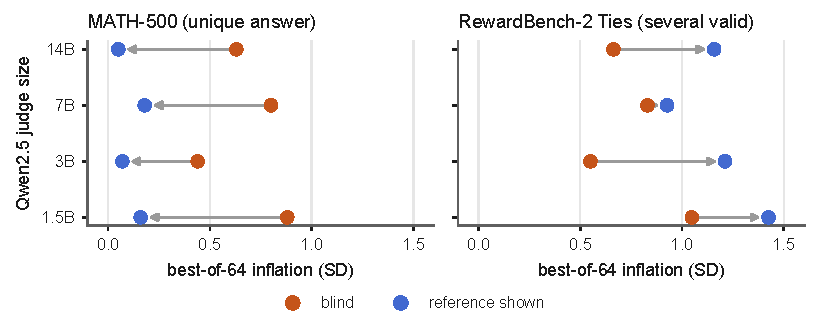
\includegraphics[width=\textwidth]{figures/figA_inversion.pdf}
\caption{\textbf{Showing the reference lowers inflation on MATH-500 and raises it on Ties.} Best-of-64 inflation for blind (orange) and referenced (blue) Qwen2.5 judges, 105 MATH-500 problems and 51 Ties tasks.}
\label{fig:inversion}
\end{figure}

In accuracy units, the reference raises MATH-500 selection accuracy at every judge size (\cref{tab:acc-math}). The local copies of these MATH-500 score files that we first used for this readout were misaligned with the candidate pool; all MATH-500 analyses reported here use byte-exact copies of the aligned files, as recorded in a registration amendment made before the remaining readouts.

\begin{table}[h]
\centering
\footnotesize
\begin{adjustbox}{max width=\linewidth}\begin{tabular}{lccc}
\toprule
Qwen2.5 judge & Blind & With reference & Change (points) \\
\midrule
1.5B & 55.2\% & 99.1\% & $+43.8$ {\scriptsize$[+34.3,+53.3]$} \\
3B & 57.1\% & 96.2\% & $+39.1$ {\scriptsize$[+30.5,+48.6]$} \\
7B & 67.6\% & 98.1\% & $+30.5$ {\scriptsize$[+21.9,+40.0]$} \\
14B & 67.6\% & 95.2\% & $+27.6$ {\scriptsize$[+18.1,+37.1]$} \\
\bottomrule
\end{tabular}
\end{adjustbox}
\caption{MATH-500 selection accuracy, 105 problems (95\% CI on the change).\ph}
\label{tab:acc-math}
\end{table}

%==========================================================================================
\FloatBarrier
\section{\textsc{MACE}: audits and results}
\label{app:mace}

\textsc{MACE}~\citep{mace2026} asks factual questions whose number of correct answers is fixed by construction at $k \in \{1,2,4,6\}$. Before building the pool we audited each domain. All 2,000 Math-domain questions have correct and complete answer sets by direct computation, so the domain enters as a label-noise control. For the entity domains we measured how often a model names a valid answer missing from the shipped list: River (2.3\%) and Language (8.1\%) passed, and Region, Office, and Award (30.8\% to 43.5\%) were excluded.

\begin{table}[h]
\centering
\footnotesize
\begin{adjustbox}{max width=\linewidth}\begin{tabular}{llccc}
\toprule
Judge & Domain & $k{=}1$ & $k{>}1$ & Step \\
\midrule
Qwen2.5-7B & River + Language & $-0.97$ {\scriptsize$[-1.29,-0.67]$} & $+1.33$ {\scriptsize$[+0.79,+1.79]$} & $+2.30$ {\scriptsize$[+1.82,+2.84]$} \\
 & \quad River & $-0.82$ {\scriptsize$[-1.21,-0.50]$} & $+0.85$ {\scriptsize$[-0.01,+1.64]$} & $+1.67$ {\scriptsize$[+0.92,+2.48]$} \\
 & \quad Language & $-1.11$ {\scriptsize$[-1.55,-0.67]$} & $+1.67$ {\scriptsize$[+1.00,+2.31]$} & $+2.78$ {\scriptsize$[+2.18,+3.47]$} \\
 & Math (control) & $+0.09$ {\scriptsize$[-0.26,+0.42]$} & $+0.83$ {\scriptsize$[+0.52,+1.16]$} & $+0.75$ {\scriptsize$[+0.42,+1.04]$} \\
\addlinespace
phi-4 & River + Language & $-0.57$ {\scriptsize$[-0.84,-0.33]$} & $+0.55$ {\scriptsize$[+0.24,+0.88]$} & $+1.13$ {\scriptsize$[+0.81,+1.43]$} \\
 & \quad River & $-0.64$ {\scriptsize$[-1.00,-0.32]$} & $+0.45$ {\scriptsize$[-0.12,+0.98]$} & $+1.08$ {\scriptsize$[+0.54,+1.64]$} \\
 & \quad Language & $-0.52$ {\scriptsize$[-0.91,-0.21]$} & $+0.63$ {\scriptsize$[+0.29,+1.00]$} & $+1.15$ {\scriptsize$[+0.81,+1.54]$} \\
 & Math (control) & $-0.40$ {\scriptsize$[-0.86,+0.09]$} & $+0.54$ {\scriptsize$[+0.32,+0.77]$} & $+0.94$ {\scriptsize$[+0.71,+1.16]$} \\
\bottomrule
\end{tabular}
\end{adjustbox}
\caption{\textsc{MACE}: added inflation (\sd, 95\% CI). The step holds in each audited domain, and the math control has the same sign.\pre}
\label{tab:mace}
\end{table}

Anchoring margins at $k{>}1$ are $+6.44$ and $+5.86$ on the audited domains, against blind margins of $-0.64$ and $-0.80$. Sonnet~5 has a referenced margin of $+5.29$ there, against a blind margin of $-1.37$.

%==========================================================================================
\FloatBarrier
\section{Frontier judges}
\label{app:frontier}

\paragraph{CLI judge.}
This check called \texttt{claude -p --model sonnet} from the project directory in August 2026, so the command-line interface's default agent system prompt and project context were present, and its extended-thinking setting was the interface default, which we did not record. On 37 $k$-pool tasks, blind, the judge scored matching and non-matching valid answers $7.88$ and $7.85$ (mean per-task margin $+0.35$ \ci{-0.56}{+1.27}); with the reference, $9.83$ and $2.32$ (mean per-task margin $+7.49$ \ci{+6.62}{+8.22}). Per task, it scored 20.5\% \ci{12.6}{29.1} of correct non-matching answers at 3 or below blind and 83.3\% \ci{75.5}{90.3} with the reference; for correct matching answers the rates were 19.1\% and 0.9\%. We had predicted a smaller margin than the open judges', continuing their size trend; the comparison is not interpretable because this interface returns sampled integers while the open judges report expected scores.

\paragraph{API judges.}
Sonnet~5 reproduces the rotation (\cref{tab:rotation}), the blind-accepted filter, the masking pattern (bare reference $+3.06$, words $+3.14$, expression $+0.47$), and the \textsc{MACE} reversal. GPT-4.1 picks matching answers far more often with the reference (32 referenced-only against 1 blind-only picks) and has a margin of $+1.19$. It failed our pre-specified score-resolution screen: an average of 15.03 candidates per pool tie at its maximum score, against a bar of 3.0. Its $k$ step is $+0.27$ \ci{-0.02}{+0.61} on the $k$-pool and $-0.08$ \ci{-0.49}{+0.20} on the synthetic grid, where ties are heavier (47.0 per pool), so we report it as unresolved.

\begin{table}[h]
\centering
\footnotesize
\begin{adjustbox}{max width=\linewidth}\begin{tabular}{lcc}
\toprule
Readout & GPT-4.1 & Claude Sonnet 5 \\
\midrule
Replication pool: added inflation ($n{=}105$) & $+0.12$ {\scriptsize$[+0.02,+0.23]$} & --- \\
Replication pool: referenced-only / blind-only picks & 32 / 1 & --- \\
Replication pool: anchoring margin & $+1.19$ {\scriptsize$[+0.92,+1.50]$} & --- \\
$k$-pool: step $k{>}1$ minus $k{=}1$ & $+0.27$ {\scriptsize$[-0.02,+0.61]$} & --- \\
$k$-pool margin, reference & $+0.99$ {\scriptsize$[+0.57,+1.55]$} & $+3.00$ {\scriptsize$[+2.02,+4.02]$} \\
\quad + any-valid-answer instruction & $+0.46$ {\scriptsize$[+0.13,+0.94]$} & $+2.08$ {\scriptsize$[+1.14,+3.14]$} \\
\quad + do-not-compare instruction & $+0.59$ {\scriptsize$[+0.21,+1.12]$} & $+2.60$ {\scriptsize$[+1.59,+3.66]$} \\
$k$-pool margin, blind & $+0.09$ {\scriptsize$[-0.46,+0.74]$} & $+0.20$ {\scriptsize$[-0.46,+0.99]$} \\
\bottomrule
\end{tabular}
\end{adjustbox}
\caption{API judges (inflation in \sd, margins in points, 95\% CI). GPT-4.1's inflation and step rows are unreliable because of ties. Sonnet~5's inflation and step were not run: its tool-call scores are integers and tie under best-of-64.\pre}
\label{tab:frontier-api}
\end{table}

%==========================================================================================
\FloatBarrier
\section{Which pools inflate: composition, lures, and distance}
\label{app:composition}

\paragraph{The margin alone does not predict which tasks inflate.}
Across the 35 multi-answer tasks of the $k$-pool with usable margins, the correlation between a task's anchoring margin and its inflation is $+0.29$ for phi-4 and $+0.06$ for Qwen2.5-7B, well below the $0.82$ and $0.90$ that measurement noise would allow under a linear link.

\paragraph{A failed prediction about composition.}
In matched sub-pools of 24 samples with exactly 4 valid answers, of which $d \in \{0,1,2,4\}$ match the reference (48 tasks), we predicted that inflation would grow with $d$. It falls (\cref{tab:dose}). With no correct answer to anchor on, the referenced judge picks a valid sample 14\% and 21\% of the time at $d{=}0$, against 72\% and 79\% blind, and 58\% and 72\% of the invalid samples it picks contain the reference's answer text, against 43\% and 35\% blind.

\begin{table}[h]
\centering
\footnotesize
\begin{adjustbox}{max width=\linewidth}\begin{tabular}{lccccc}
\toprule
Judge & $d{=}0$ & $d{=}1$ & $d{=}2$ & $d{=}4$ & $d{=}4$ minus $d{=}0$ \\
\midrule
Qwen2.5-7B & $+1.18$ {\scriptsize$[+0.99,+1.37]$} & $+1.10$ {\scriptsize$[+0.95,+1.26]$} & $+0.65$ {\scriptsize$[+0.50,+0.78]$} & $-0.23$ {\scriptsize$[-0.43,-0.03]$} & $-1.41$ {\scriptsize$[-1.66,-1.15]$} \\
phi-4 & $+0.95$ {\scriptsize$[+0.82,+1.08]$} & $+0.58$ {\scriptsize$[+0.45,+0.72]$} & $+0.22$ {\scriptsize$[+0.13,+0.31]$} & $-0.44$ {\scriptsize$[-0.56,-0.33]$} & $-1.39$ {\scriptsize$[-1.56,-1.22]$} \\
\bottomrule
\end{tabular}
\end{adjustbox}
\caption{Added inflation by the number $d$ of valid samples matching the reference (\sd, 95\% CI).\pre}
\label{tab:dose}
\end{table}

\paragraph{Lures and a selection model.}
A second design crossed $d \in \{0,2,4\}$ with the number of invalid samples that resemble the reference, $\ell \in \{0,3,6\}$ (14-sample sub-pools, 24 tasks). Adding lures at $d{=}0$ lowers the referenced judge's valid-pick rate ($-0.31$ and $-0.38$). A model fit per judge,
$S_{\text{ref}} \approx \beta S_{\text{blind}} + \lambda\,\mathbb{I}[\text{matches } r] + \gamma\,\mathbb{I}[\text{invalid lure}]$,
gives match bonuses $\lambda = +4.3$ and $+3.5$ points and lure bonuses $\gamma = +1.4$ and $+1.7$, and reproduces the nine-cell inflation surface out of sample at Spearman $0.80$ and $0.85$. With no lures and no matching valid answers the referenced judge still inflates ($+0.68$ and $+0.66$), which the model attributes to $\beta \approx 0.5$ to $0.7$: a referenced score keeps only part of the blind score's information. Because $\beta<1$ partly reflects measurement attenuation, we read it descriptively.

\paragraph{Distance.}
Among valid answers that do not match the reference, the penalty does not grow with numeric distance from it, for either judge. Including matching samples, the slope is $-3.38$ and $-2.18$ points per unit distance, driven by the step at exact equality; blind slopes are near zero.

%==========================================================================================
\FloatBarrier
\section{Mechanism details}
\label{app:mechanism}

\begin{table}[h]
\centering
\footnotesize
\setlength{\tabcolsep}{3pt}
\begin{adjustbox}{max width=\linewidth}\begin{tabular}{llcccc}
\toprule
Judge & Rubric & Numeral & Words & Expression & Worked: visible $\to$ masked \\
\midrule
Qwen2.5-7B & $a$ & $+4.62$ {\scriptsize$[+4.32,+4.96]$} & $+2.88$ {\scriptsize$[+2.47,+3.28]$} & $+0.29$ {\scriptsize$[+0.07,+0.49]$} & $+2.97$ {\scriptsize$[+2.01,+4.06]$} $\to$ $+0.05$ {\scriptsize$[-0.52,+0.63]$} \\
 & $b$ & $+5.99$ {\scriptsize$[+5.69,+6.29]$} & $+4.60$ {\scriptsize$[+4.14,+5.03]$} & $+0.35$ {\scriptsize$[+0.12,+0.56]$} & $+4.62$ {\scriptsize$[+3.57,+5.78]$} $\to$ $+0.31$ {\scriptsize$[-0.46,+1.13]$} \\
phi-4 & $a$ & $+3.79$ {\scriptsize$[+3.48,+4.11]$} & $+3.68$ {\scriptsize$[+3.27,+4.06]$} & $+0.89$ {\scriptsize$[+0.64,+1.13]$} & $+3.51$ {\scriptsize$[+3.06,+4.01]$} $\to$ $-0.49$ {\scriptsize$[-1.27,+0.26]$} \\
 & $b$ & $+3.11$ {\scriptsize$[+2.83,+3.39]$} & $+3.01$ {\scriptsize$[+2.71,+3.37]$} & $+0.63$ {\scriptsize$[+0.45,+0.82]$} & $+2.84$ {\scriptsize$[+2.40,+3.28]$} $\to$ $-0.45$ {\scriptsize$[-1.11,+0.12]$} \\
\bottomrule
\end{tabular}
\end{adjustbox}
\caption{Masking suite: anchoring margin by how the reference is written (0--10 scale, 95\% CI). Numeral, words, and expression use 93 replication-pool tasks; the worked-solution columns use 21 $k$-pool tasks with a single-number answer.\pre}
\label{tab:masking}
\end{table}

\paragraph{Decode cost.}
We kept the answer an integer and re-encoded the reference with one, two, or three reversible steps (a digit shift; then base64; then string reversal), stating the decoding rule each time. We had predicted a graded decline; the margin instead collapsed at the first step and stayed at zero (\cref{tab:cipher}). Every encoded prompt announced that the reference had been encoded, and that framing may explain the collapse by itself: ``30+1'', a comparable single step without such framing, shrank the margin only partly.

\begin{table}[h]
\centering
\footnotesize
\begin{adjustbox}{max width=\linewidth}\begin{tabular}{lcccc}
\toprule
Judge & Plain reference & One decode step & Two steps & Three steps \\
\midrule
Qwen2.5-7B & $+4.62$ {\scriptsize$[+4.32,+4.96]$} & $-0.18$ {\scriptsize$[-0.44,+0.08]$} & $-0.28$ {\scriptsize$[-0.57,+0.00]$} & $-0.27$ {\scriptsize$[-0.56,+0.00]$} \\
phi-4 & $+3.79$ {\scriptsize$[+3.46,+4.12]$} & $-0.02$ {\scriptsize$[-0.07,+0.03]$} & $+0.00$ {\scriptsize$[+0.00,+0.01]$} & $+0.01$ {\scriptsize$[+0.00,+0.01]$} \\
\bottomrule
\end{tabular}
\end{adjustbox}
\caption{Anchoring margin with the reference encoded by one to three stated decoding steps (0--10 scale, 95\% CI, 93 tasks).\pre}
\label{tab:cipher}
\end{table}

\paragraph{Solution route.}
Holding the reference answer fixed and rotating its derivation to a different method moves the identical sample's score by $-0.32$ and $-0.40$ points for Qwen2.5-7B and $-0.02$ for phi-4. Three of four cells exclude zero, so the prediction of no effect is falsified as stated, but the effects are 20 to 400 times smaller than answer rotation, and a preference for samples whose own route matches the shown one appears in one of four cells.

%==========================================================================================
\FloatBarrier
\section{Code and the answer-format continuum}
\label{app:code}

\paragraph{MBPP.}
Three conditions score identical samples with identical judges: blind, the test suite as reference, and the canonical solution as reference. Contrasts use the 58 tasks inside the pass-rate band shared by all three.

\begin{table}[h]
\centering
\footnotesize
\begin{tabular}{lccc}
\toprule
Judge & Test suite vs.\ blind & Canonical solution vs.\ blind & Solution minus test suite \\
\midrule
Qwen2.5-7B  & $-0.535$ \ci{-0.811}{-0.244} & $-0.342$ \ci{-0.737}{+0.041} & $+0.193$ \ci{-0.112}{+0.475} \\
Qwen2.5-14B & $-0.658$ \ci{-0.965}{-0.373} & $-0.567$ \ci{-0.827}{-0.287} & $+0.091$ \ci{-0.102}{+0.277} \\
\bottomrule
\end{tabular}
\caption{MBPP: paired inflation differences (\sd, 95\% CI), 58 tasks. Negative values mean the reference lowers inflation.\pre}
\label{tab:code}
\end{table}

Among valid samples, the correlation between token similarity to the canonical solution and the judge's score is $+0.164$ \ci{+0.072}{+0.256} for the 7B judge and $+0.084$ \ci{-0.005}{+0.168} for the 14B judge with the solution shown, against $-0.061$ and $-0.070$ blind.

\paragraph{The continuum.}
Each of 25 new tasks was requested in four formats with the content fixed. Three disclosures apply. The margin predictions at the pair and JSON formats could not be evaluated, because a valid sample rarely matches the sampled reference exactly in those formats (7 and 1 usable tasks). Program outputs cluster (a median of two distinct returned lists per task), so the program format has few distinct valid answers. And the registered program checker executed the last code block of a reply, which scored 387 of 1,600 samples invalid when a usage line such as \texttt{print(f())} followed the definition of \texttt{f}; re-scoring with the last block that defines \texttt{f} flipped 330 of them to valid and none the other way. \Cref{tab:continuum} uses the corrected labels. Under the registered labels the program-format values were $+0.27$ \ci{+0.13}{+0.40} and $-0.06$ \ci{-0.22}{+0.11}; no registered verdict changes.

\begin{table}[h]
\centering
\footnotesize
\setlength{\tabcolsep}{3pt}
\begin{adjustbox}{max width=\linewidth}\begin{tabular}{llcccc}
\toprule
Judge & Readout & Integer & Pair & JSON & Program \\
\midrule
Qwen2.5-7B & added inflation ($n{=}25$) & $+1.66$ {\scriptsize$[+1.34,+2.03]$} & $+1.35$ {\scriptsize$[+1.06,+1.68]$} & $+0.71$ {\scriptsize$[+0.40,+1.02]$} & $+0.13$ {\scriptsize$[+0.01,+0.24]$} \\
 & anchoring margin & $+4.65$ {\scriptsize($n{=}17$)} & $+5.45$ {\scriptsize($n{=}7$)} & --- {\scriptsize($n{=}1$)} & $+0.64$ {\scriptsize($n{=}19$)} \\
phi-4 & added inflation ($n{=}25$) & $+1.35$ {\scriptsize$[+1.06,+1.65]$} & $+0.98$ {\scriptsize$[+0.77,+1.21]$} & $+0.94$ {\scriptsize$[+0.56,+1.30]$} & $-0.37$ {\scriptsize$[-0.49,-0.27]$} \\
 & anchoring margin & $+3.22$ {\scriptsize($n{=}17$)} & $+3.79$ {\scriptsize($n{=}7$)} & --- {\scriptsize($n{=}1$)} & $+0.88$ {\scriptsize($n{=}19$)} \\
\bottomrule
\end{tabular}
\end{adjustbox}
\caption{Answer-format continuum: added inflation (\sd, 95\% CI) and anchoring margins with the number of usable tasks; margins on fewer than five tasks are omitted.\pre}
\label{tab:continuum}
\end{table}

%==========================================================================================
\FloatBarrier
\section{Training runs}
\label{app:dpo}

Arms trained Llama-3.1-8B-Instruct with LoRA-DPO~\citep{rafailov2023dpo,hu2022lora} on identical tasks and hyperparameters, differing only in the judge protocol that labeled the preference pairs: the referenced Qwen2.5-7B judge, the same judge under blind-then-reveal, and in run 3 the blind judge. Each arm's manipulation check required its own judge's score to rise. The \emph{wedge} is the rise in own-judge score (points) minus ten times the rise in accuracy, so both terms are on the 0--10 scale.

\begin{table}[h]
\centering
\footnotesize
\setlength{\tabcolsep}{3pt}
\begin{adjustbox}{max width=\linewidth}\begin{tabular}{llccc}
\toprule
Run & Arm & Own-judge gain (gate) & Score--accuracy gap (points) & Held-out accuracy change \\
\midrule
1 (4 ep., lr $2{\times}10^{-5}$) & reference & $+1.76$ {\scriptsize$[+1.47,+2.01]$} & $+4.13$ {\scriptsize$[+3.50,+4.78]$} & $-0.228$ {\scriptsize$[-0.269,-0.189]$} \\
 & blind-then-reveal & $-1.04$ {\scriptsize$[-1.36,-0.72]$} & $+1.48$ {\scriptsize$[+0.99,+1.97]$} & $-0.049$ {\scriptsize$[-0.091,-0.010]$} \\
\addlinespace
3 (2 ep., lr $10^{-5}$) & reference & $+0.34$ {\scriptsize$[+0.10,+0.57]$} & $+1.16$ {\scriptsize$[+0.67,+1.61]$} & $-0.110$ {\scriptsize$[-0.149,-0.074]$} \\
 & blind-then-reveal & $-0.99$ {\scriptsize$[-1.23,-0.74]$} & $+1.10$ {\scriptsize$[+0.62,+1.58]$} & $-0.073$ {\scriptsize$[-0.107,-0.040]$} \\
 & blind judge & $-2.43$ {\scriptsize$[-2.78,-2.12]$} & $+1.90$ {\scriptsize$[+1.41,+2.43]$} & $-0.125$ {\scriptsize$[-0.159,-0.092]$} \\
\bottomrule
\end{tabular}
\end{adjustbox}
\caption{Training runs. Only the reference arm passed its manipulation check. Run 2 (1 epoch, lr $5{\times}10^{-6}$) moved neither judge and is omitted.\pre}
\label{tab:dpo}
\end{table}

The reference arm did not copy the reference more often; its exact-reference rate fell. It wrote longer answers and mostly stopped using the boxed format, and almost all of its unboxed answers were also wrong (390 of 405 on training tasks), so this is a joint failure of format and correctness, not an extraction artifact (\cref{tab:dpo-profile}). Held-out accuracy fell in every arm, including the controls. In run 1 both arms drifted toward verbosity, which the blind-first judge penalizes; in run 2 neither arm moved; before run 3 we adopted a stopping rule allowing one more setting, and in run 3 the reveal and blind arms lost score and accuracy together. We stopped there, so whether blind-then-reveal protects a trained policy, and whether the reference specifically causes the damage, remain open.

\begin{table}[h]
\centering
\scriptsize
\setlength{\tabcolsep}{3pt}
\begin{adjustbox}{max width=\linewidth}\begin{tabular}{lcccccc}
\toprule
Policy (items) & Accuracy & Boxed answers & Mean length (chars) & 4-gram repetition & Unboxed and valid & Unboxed and invalid \\
\midrule
Base, train (60) & 0.412 & 0.581 & 1492 & 0.080 & 3 & 198 \\
Reference arm, train (60) & 0.175 & 0.156 & 2476 & 0.062 & 15 & 390 \\
Reveal arm, train (60) & 0.331 & 0.365 & 3840 & 0.032 & 0 & 305 \\
Base, held out (120) & 0.457 & 0.613 & 1376 & 0.080 & 13 & 359 \\
Reference arm, held out (120) & 0.229 & 0.174 & 2187 & 0.064 & 57 & 736 \\
Reveal arm, held out (120) & 0.408 & 0.455 & 3458 & 0.041 & 4 & 519 \\
\bottomrule
\end{tabular}
\end{adjustbox}
\caption{Generation profile of the run-1 policies.\ph}
\label{tab:dpo-profile}
\end{table}

%==========================================================================================
\FloatBarrier
\section{Mitigations in full}
\label{app:mitigation}

\paragraph{Instructions and several references.}
On the synthetic grid at $k{=}16$, the any-valid-answer instruction closes phi-4's margin ($+1.91 \to +0.03$), shrinks Qwen2.5-14B's ($+3.34 \to +1.21$), and leaves smaller judges unmoved or worse (Qwen2.5-1.5B, rubric~$a$: $+3.58 \to +4.54$). Showing $\min(3,k)$ valid references removes the margin toward the original reference on the Qwen-generated grid without restoring blind-level inflation, and largely fails for Qwen2.5-7B on the Llama-generated grid.

\paragraph{Worked references.}
With a short worked solution in the reference slot on the $k$-pool, the margin falls from $+5.17$ to $+3.73$ (Qwen2.5-7B) and from $+4.20$ to $+3.67$ (phi-4), and added inflation falls from $+1.50$ to $+1.08$ and from $+1.07$ to $+0.77$.

\paragraph{Blind-then-reveal on unique answers.}
A later pre-specified experiment ran blind-then-reveal on the 105 MATH-500 problems (\cref{tab:r2a}). The first call reproduces the frozen blind scores ($r=0.991$ and $0.973$), so the comparison is on aligned data.

\begin{table}[h]
\centering
\footnotesize
\begin{adjustbox}{max width=\linewidth}\begin{tabular}{lccccc}
\toprule
Judge & Blind & Reference & Blind, then reveal & Reveal minus reference (points) & Call-1 vs.\ frozen blind $r$ \\
\midrule
Qwen2.5-7B & 67.6\% & 98.1\% & 95.2\% & $-2.9$ {\scriptsize$[-8.6,+1.9]$} & 0.991 \\
Qwen2.5-14B & 67.6\% & 95.2\% & 93.5\% & $-1.7$ {\scriptsize$[-7.3,+3.3]$} & 0.973 \\
\bottomrule
\end{tabular}
\end{adjustbox}
\caption{MATH-500 selection accuracy under three protocols, best of 64, rubric-$a$ selection.\pre}
\label{tab:r2a}
\end{table}

\paragraph{Blind-then-reveal across judges.}
\Cref{tab:coverage} gives the preregistered coverage extension in inflation units, and \cref{tab:acc-kpool} gives all five $k$-pool judges in accuracy units.

\begin{table}[h]
\centering
\scriptsize
\setlength{\tabcolsep}{3pt}
\begin{adjustbox}{max width=\linewidth}\begin{tabular}{lccccc}
\toprule
Judge & Reference, $k{=}1$ & Reference, $k{>}1$ & Blind-then-reveal, $k{>}1$ & Validity gate, $k{>}1$ & Reveal minus reference \\
\midrule
Qwen2.5-14B & $-0.30$ {\scriptsize$[-0.73,+0.13]$} & $+0.98$ {\scriptsize$[+0.64,+1.33]$} & $+0.23$ {\scriptsize$[+0.10,+0.37]$} & $+0.30$ {\scriptsize$[+0.18,+0.43]$} & $-0.75$ {\scriptsize$[-1.05,-0.46]$} \\
gemma-2-9b & $-0.05$ {\scriptsize$[-0.14,+0.04]$} & $+1.43$ {\scriptsize$[+1.15,+1.68]$} & $+1.23$ {\scriptsize$[+0.94,+1.52]$} & $+0.61$ {\scriptsize$[+0.48,+0.76]$} & $-0.20$ {\scriptsize$[-0.34,-0.05]$} \\
Mistral-7B & $+0.07$ {\scriptsize$[-0.01,+0.13]$} & $+0.03$ {\scriptsize$[-0.03,+0.08]$} & $-0.04$ {\scriptsize$[-0.08,-0.01]$} & $+0.09$ {\scriptsize$[-0.01,+0.19]$} & $-0.07$ {\scriptsize$[-0.12,-0.02]$} \\
\bottomrule
\end{tabular}
\end{adjustbox}
\caption{Judge-coverage extension on the $k$-pool (\sd, 95\% CI).\osf}
\label{tab:coverage}
\end{table}

\paragraph{Variants of the reveal call.}
\Cref{tab:m1variants} gives the pre-specified variants in inflation units (58 multi-answer tasks from the $k$-pool and replication pool) and \cref{tab:acc-variants} in accuracy units (39 $k$-pool tasks). In inflation, removing the displayed score restores the harm for all three judges. For Qwen2.5-7B, neutral wording costs $+0.51$ \ci{+0.28}{+0.73} of protection, which falsified our equivalence prediction for that judge, and another judge's score gives $+0.38$ against $+0.01$ for its own. For gemma-2-9b, another judge's score costs $+0.17$ \ci{+0.01}{+0.38} relative to its own. gemma also puts the lowest weight on its own blind score in the selection model of \cref{app:composition} ($\beta = 0.34$, against $0.51$ and $0.69$), a consistent ordering on only four eligible tasks. In accuracy units the variant contrasts are imprecise.

\begin{table}[h]
\centering
\footnotesize
\setlength{\tabcolsep}{3pt}
\begin{adjustbox}{max width=\linewidth}\begin{tabular}{lcccc}
\toprule
Judge & Own blind score & No score & Neutral wording & Other judge's score \\
\midrule
Qwen2.5-7B & $+0.01$ {\scriptsize$[-0.24,+0.29]$} & $+1.42$ {\scriptsize$[+1.10,+1.73]$} & $+0.53$ {\scriptsize$[+0.29,+0.80]$} & $+0.38$ {\scriptsize$[+0.12,+0.60]$} \\
phi-4 & $+0.12$ {\scriptsize$[-0.07,+0.29]$} & $+0.36$ {\scriptsize$[+0.15,+0.55]$} & $+0.08$ {\scriptsize$[-0.11,+0.28]$} & $+0.09$ {\scriptsize$[-0.09,+0.26]$} \\
gemma-2-9b & $+1.21$ {\scriptsize$[+0.91,+1.51]$} & $+1.41$ {\scriptsize$[+1.12,+1.68]$} & $+1.30$ {\scriptsize$[+1.02,+1.60]$} & $+1.48$ {\scriptsize$[+1.17,+1.80]$} \\
\bottomrule
\end{tabular}
\end{adjustbox}
\caption{Reveal-call variants: added inflation over blind (\sd, 95\% CI), 58 tasks.\pre}
\label{tab:m1variants}
\end{table}

\begin{table}[h]
\centering
\footnotesize
\setlength{\tabcolsep}{3pt}
\begin{adjustbox}{max width=\linewidth}\begin{tabular}{lccccc}
\toprule
Judge & Reference & Reveal, own score & Reveal, no score & Reveal, neutral wording & Reveal, other judge's score \\
\midrule
Qwen2.5-7B & $-30.8$ {\scriptsize$[-46.2,-17.9]$} & $-10.3$ {\scriptsize$[-25.6,+5.1]$} & $-23.1$ {\scriptsize$[-38.5,-7.7]$} & $-10.3$ {\scriptsize$[-25.6,+2.6]$} & $-7.7$ {\scriptsize$[-20.5,+5.1]$} \\
phi-4 & $-20.5$ {\scriptsize$[-35.9,-5.1]$} & $-15.4$ {\scriptsize$[-28.2,-2.6]$} & $-15.4$ {\scriptsize$[-28.2,-2.6]$} & $-7.7$ {\scriptsize$[-20.5,+2.6]$} & $-7.7$ {\scriptsize$[-18.0,+2.6]$} \\
gemma-2-9b & $-17.9$ {\scriptsize$[-30.8,-7.7]$} & $-12.8$ {\scriptsize$[-25.6,-2.6]$} & $-10.3$ {\scriptsize$[-20.5,+0.0]$} & $-20.5$ {\scriptsize$[-33.3,-7.7]$} & $-17.9$ {\scriptsize$[-30.8,-5.1]$} \\
\bottomrule
\end{tabular}
\end{adjustbox}
\caption{Reveal-call variants: change in selection accuracy relative to blind, in points (95\% CI), 39 $k$-pool tasks at $k{>}1$.\ph}
\label{tab:acc-variants}
\end{table}

\paragraph{The validity gate backfires for one judge.}
A second preregistered protocol multiplies the blind score by a separate call's probability that the candidate is valid, with the reference shown to that call as one valid example. For phi-4 it removes the inflation. For Qwen2.5-7B it raises the $k{=}2$ margin from $+5.02$ to $+6.62$, because the validity call itself anchors: its probability averages $0.998$ for matching valid answers and $0.422$ for non-matching valid ones.

\paragraph{A free screen rejects broken judges and certifies nothing.}
Mistral-7B's null harm in inflation units is a resolution artifact. Its tokenizer writes every digit as two tokens, a space marker and the digit, so no score token is ever captured and every score is the integer parsed from its greedy reply. Its scores therefore take only 11 distinct values, 52.6\% of its referenced scores are exactly 10, and with the reference an average of 32.1 of its 64 candidates tie at the maximum, so selection cannot act on its anchoring (margin $+1.38$). Counting distinct values and ties catches this (\cref{tab:resolution}). Ministral-8B passes the distinct-value check but has a score standard deviation of $0.55$ around a mean of $4.73$, is essentially uncorrelated with validity, and picks a valid answer 21.7\% of the time against a 38.6\% random baseline. Passing the screen certifies nothing: gemma-2-9b passes easily and is the most anchored of the five $k$-pool judges.

\begin{table}[h]
\centering
\footnotesize
\begin{adjustbox}{max width=\linewidth}\begin{tabular}{lcccc}
\toprule
Judge & Distinct score values & Blind ties at max (of 64) & Blind selection accuracy & Anchoring margin \\
\midrule
Qwen2.5-7B & 2506 & 1.0 & 0.767 & $+5.17$ \\
phi-4 & 2511 & 1.0 & 0.850 & $+4.20$ \\
Qwen2.5-14B & 2491 & 1.0 & 0.750 & $+4.06$ \\
gemma-2-9b & 2751 & 1.0 & 0.750 & $+5.32$ \\
Mistral-7B & 11 & 17.8 & 0.564 & $+1.38$ \\
\bottomrule
\end{tabular}
\end{adjustbox}
\caption{Score-resolution screen on the $k$-pool; tie counts and selection accuracy use blind scores.\pre}
\label{tab:resolution}
\end{table}

%==========================================================================================
\FloatBarrier
\section{Reasoning, verification, and a natural multi-answer pool}
\label{app:reasoning}

\paragraph{Thinking on versus off.}
This pre-specified experiment reran the Qwen3-8B protocol of \cref{app:rotation} (rubric~$a$ ending in a ``Score: N'' line, temperature 0.6, top-p 0.95, top-k 20, up to 4,096 new tokens) with the chat template's thinking switch off and nothing else changed. The pools are the rotation subsample and the 16-sample $k$-subsample of \cref{app:rotation}, plus a \textsc{MACE} subsample: every River or Language task with $k{>}1$ that has both matching and non-matching valid samples, with up to four samples each of matching-valid, non-matching-valid, and invalid answers (81 tasks, 825 samples). Twelve of 1,200 blind thinking-off replies on the $k$-subsample had no parseable score; none did elsewhere. \Cref{tab:toggle} gives the results.

\begin{table}[h]
\centering
\footnotesize
\setlength{\tabcolsep}{3pt}
\begin{adjustbox}{max width=\linewidth}\begin{tabular}{llccc}
\toprule
Task type & Readout & Thinking off & Thinking on & Tokens (off / on) \\
\midrule
Arithmetic (rotation) & moved onto & $+0.567$ {\scriptsize$[+0.414,+0.747]$} & $-0.006$ {\scriptsize$[-0.017,+0.000]$} & 159 / 569 \\
 & no longer matches & $-0.694$ {\scriptsize$[-0.918,-0.471]$} & $+0.011$ {\scriptsize$[+0.000,+0.032]$} & \\
 & matches neither & $-0.035$ {\scriptsize$[-0.209,+0.142]$} & $-0.003$ {\scriptsize$[-0.009,+0.000]$} & \\
Arithmetic ($k$-subsample) & margin, ref $-$ blind & $+1.18$ {\scriptsize$[+0.25,+2.38]$} & $+0.06$ {\scriptsize$[-0.10,+0.26]$} & 193 / 1009 \\
Factual (MACE subsample) & margin, ref $-$ blind & $+6.16$ {\scriptsize$[+5.23,+7.15]$} & $+3.62$ {\scriptsize$[+2.55,+4.75]$} & 80 / 631 \\
 & false rejections, ref $-$ blind & $+44.3$ {\scriptsize$[+36.9,+52.3]$} & $+21.6$ {\scriptsize$[+13.3,+29.9]$} & \\
\bottomrule
\end{tabular}
\end{adjustbox}
\caption{Qwen3-8B with thinking off and on, same weights and prompt. Rotation rows: change in score of identical valid text (points). Margin rows: referenced-minus-blind anchoring margin (points). False rejections: share of non-matching valid answers scored 3 or below, referenced minus blind (points). 95\% CI; mean generated tokens.\pre}
\label{tab:toggle}
\end{table}

With thinking on, valid rotation samples receive 10 in 99.8\% of referenced replies and 96.2\% of blind ones; with thinking off, in 79.2\% and 76.9\%. The thinking judge's arithmetic scores therefore sit at the top of the scale whether or not the reference agrees, which is what verification looks like on these tasks and leaves no room for a reference to move them. On \textsc{MACE} its valid answers average 7.96 with the reference and 8.18 blind, away from the ceiling, and the anchoring returns. These diagnostics are post hoc.

\paragraph{Sonnet~5 with and without thinking.}
A pre-specified three-arm design tested the same contrast on a frontier judge through the Claude command-line tool (default system prompt replaced, no tools, an empty working directory, subscription login), on 60 replication-pool tasks with one sample each that gains, loses, or keeps neither reference under rotation. The score-only arm, with thinking off, anchors: $+3.57$ \ci{+2.57}{+4.55} for text the reference moves onto, $-2.85$ \ci{-3.85}{-1.92} for text it moves off, and $-0.07$ \ci{-1.18}{+1.10} for text matching neither, with 26.7\% \ci{20.4}{33.3} of correct non-matching answers scored 3 or below and 52 to 58 output tokens per reply. The visible-reasoning and thinking arms were stopped partway by the subscription's monthly usage limit (the visible arm finished only its original-reference condition, and the thinking arm has no data), so their three predictions are not scored, and we did not complete them through a different interface.

\paragraph{End to end on \textsc{MACE}.}
The last pre-specified experiment measured selection accuracy on the benchmark's natural mix of $k$: all 133 River and Language tasks in the pass-rate band (34 with $k{=}1$, 99 with $k{>}1$), best of 64, rubric-$a$ selection. Blind and referenced scores are the frozen files of \cref{app:mace}, whose blind scores correlate with validity at $0.361$ (Qwen2.5-7B) and $0.477$ (phi-4); blind-then-reveal and the validity gate were run new with the prompts of \cref{app:setup}. We predicted that the reference would lower accuracy at $k{>}1$, that blind-then-reveal would beat it there, and that blind-then-reveal would be at least as accurate over the natural mix. All three predictions failed for both judges (\cref{tab:mace-accuracy}). The anchoring on these questions is large (\cref{app:mace}), but blind judges that verify factual answers this poorly gain more from the reference's help against wrong answers than they lose to its pull away from correct ones.

\begin{table}[h]
\centering
\footnotesize
\setlength{\tabcolsep}{3pt}
\begin{adjustbox}{max width=\linewidth}\begin{tabular}{llcccccc}
\toprule
Judge & Tasks & Blind & Reference & Reveal & Validity gate & Reference $-$ blind & Reveal $-$ reference \\
\midrule
Qwen2.5-7B & $k{=}1$ (34) & 67.7 & 100.0 & 91.2 & 91.2 & $+32.4$ {\scriptsize$[+17.6,+47.1]$} & $-8.8$ {\scriptsize$[-20.6,+0.0]$} \\
 & $k{>}1$ (99) & 86.9 & 88.9 & 87.9 & 91.9 & $+2.0$ {\scriptsize$[-5.1,+9.1]$} & $-1.0$ {\scriptsize$[-7.1,+6.1]$} \\
 & all (133) & 82.0 & 91.7 & 88.7 & 91.7 & $+9.8$ {\scriptsize$[+2.3,+17.3]$} & $-3.0$ {\scriptsize$[-8.3,+2.3]$} \\
\addlinespace
phi-4 & $k{=}1$ (34) & 73.5 & 100.0 & 100.0 & 82.3 & $+26.5$ {\scriptsize$[+11.8,+41.2]$} & $+0.0$ {\scriptsize$[+0.0,+0.0]$} \\
 & $k{>}1$ (99) & 87.9 & 93.9 & 91.9 & 90.9 & $+6.1$ {\scriptsize$[-1.0,+13.1]$} & $-2.0$ {\scriptsize$[-6.1,+2.0]$} \\
 & all (133) & 84.2 & 95.5 & 94.0 & 88.7 & $+11.3$ {\scriptsize$[+5.2,+18.1]$} & $-1.5$ {\scriptsize$[-4.5,+1.5]$} \\
\bottomrule
\end{tabular}
\end{adjustbox}
\caption{\textsc{MACE} River and Language: best-of-64 selection accuracy (\%) by protocol, and differences in points (95\% CI).\pre}
\label{tab:mace-accuracy}
\end{table}

%==========================================================================================
\FloatBarrier
\section{A pilot on combinatorial constraint problems}
\label{app:mathconstraint}

Our own pools come from arithmetic constraint families. To check whether rotation and margins depend on that, we ran a pre-specified pilot on MathConstraint~\citep{mathconstraint2026}, a third-party benchmark of solver-verified combinatorial puzzles. Llama-3.1-8B-Instruct and Qwen2.5-32B-Instruct (with a worked example) solved none of 8 attempts past the smallest size, so a Claude model generated candidate solutions, each re-verified with exact checkers. It solved all 13 attempted items. Magic sequences turned out to be essentially unique past the smallest size, so the tests use all-interval series, which have several solutions at every size tried.

Rotating the reference between two valid solutions moves a fixed candidate by $+3.46$ \ci{+2.71}{+4.09} and $+3.93$ \ci{+3.42}{+4.40} for Qwen2.5-7B (rubrics $a$, $b$) and $+5.01$ \ci{+4.38}{+5.54} and $+3.90$ \ci{+3.27}{+4.49} for phi-4, and the margin is positive on all 9 eligible items for both judges. A follow-up used all six pairs of valid answers per item: $+3.21$ \ci{+2.92}{+3.51} and $+3.53$ \ci{+3.27}{+3.81} for Qwen2.5-7B and $+5.04$ \ci{+4.79}{+5.28} and $+4.10$ \ci{+3.84}{+4.36} for phi-4 (96 observations each). An invalid answer that differs from the reference by one adjacent swap scores higher than an unrelated invalid answer by $+3.47$ \ci{+2.31}{+4.52} and $+1.42$ \ci{+0.77}{+2.14}. Sonnet~5 shows the rotation ($+4.38$ \ci{+1.88}{+6.88}) and a margin of $+6.41$ \ci{+3.70}{+8.74}.

Four pre-specified attempts tested selection on this domain. The first two failed for diagnosed reasons: mixing a few valid solutions into many obviously broken attempts recreated the unique-answer case, and replacing the broken attempts with a second valid solution ran into a solution so regular that judges preferred it even blind. The third used two unstructured valid solutions and a near-miss invalid variant of each, and also failed: with the reference shown, both judges picked the candidate identical to the reference in all 16 cases. In all three designs the reference's own text was one of the candidates, so its top score shows only that a judge recognizes the string it was shown. The fourth attempt removed that candidate and asked whether showing one valid solution as the reference makes judges prefer a near-miss variant of it over a different valid solution. Both judges moved in the predicted direction (the valid pick rate fell from 0.625 to 0.375 for Qwen2.5-7B and from 0.500 to 0.375 for phi-4), but with 8 items neither interval excludes zero, so selection on this domain remains unresolved.
